%\documentclass[iop]{emulateapj}
\documentclass[aps, pre, onecolumn, nofootinbib, notitlepage, groupedaddress, amsfonts, amssymb, amsmath, longbibliography]{revtex4-1}
\usepackage{graphicx}
\usepackage{hyperref}
\usepackage{xcolor}
\hypersetup{
    colorlinks,
    linkcolor={red!50!black},
    citecolor={blue!50!black},
    urlcolor={blue!80!black}
}
\usepackage{bm}
\usepackage{natbib}
\usepackage{longtable}
\LTcapwidth=0.87\textwidth

\newcommand{\Div}[1]{\ensuremath{\nabla\cdot\left( #1\right)}}
\newcommand{\angles}[1]{\ensuremath{\left\langle #1 \right\rangle}}
\newcommand{\grad}{\ensuremath{\nabla}}
\newcommand{\RB}{Rayleigh-B\'{e}nard }
\newcommand{\stressT}{\ensuremath{\bm{\bar{\bar{\Pi}}}}}
\newcommand{\lilstressT}{\ensuremath{\bm{\bar{\bar{\sigma}}}}}
\newcommand{\nrho}{\ensuremath{n_{\rho}}}
\newcommand{\approptoinn}[2]{\mathrel{\vcenter{
	\offinterlineskip\halign{\hfil$##$\cr
	#1\propto\cr\noalign{\kern2pt}#1\sim\cr\noalign{\kern-2pt}}}}}

\newcommand{\appropto}{\mathpalette\approptoinn\relax}

\newcommand\mnras{{MNRAS}}%

\begin{document}
\title{BVP Methods}

\maketitle


\section{Brief description of method}
In a really simple sense, this is the procedure that is being done when I do the
``BVP solve'' for getting a more converged atmosphere.
\begin{enumerate}
\item Start up IVP, and run it.
\item Once the flows hit Re = 1, wait some time, $t_{\text{transient}}$.
\item After $t_{\text{transient}}$, start taking horizontal and time averages of
specified profiles in the atmosphere.
\item Once the profiles are converged (the change in the profiles at the next timestep
change, on average, less than $f$, where $f$ is a fraction.  If $f=0.01$, the profiles
change no more than 1\% from the previous timestep.), feed them into a 1D problem. 
\item In the 1D problem, adjust the profiles from the atmosphere intelligently.  Feed
those profiles into a BVP that obeys the same thermal boundary conditions as the IVP,
then adjust the mean thermal profile of the IVP atmosphere with the result of the BVP.
\item Keep running the IVP.  If desired, wait some time, $t_{\text{equil}}$, and then restart
from step 3.

\section{More thorough write-up, Boussinesq convection}
In boussinesq convection, the time-steady energy equation can be written as
$$
\Div{ \bm{u} T - \kappa \grad T} = 0
$$
When we take horizontal averages and time averages, and assume constant $\kappa$,
this equation reduces to
$$
\partial_z \angles{(w T)} - \kappa \partial^2_z \angles{(T_0 + T_1)} = 0,
$$
where angles represent a time- and horizontal average.  Further, due to symmetry,
when we take a time- and horizontal average, we find that most of the terms in the 
Rayleigh-Benard momentum equation go away.  Even if they hadn't, the main thing we want
from the momentum equation is an update to the hydrostatic balance of the atmosphere, and
that means that we need to update
$$
\partial_z \angles{p} = \angles{T_1}.
$$

So, put simply, the BVP that we need to solve in RBC is 
\begin{equation}
\begin{split}
\frac{\partial T_1}{\partial z} - T_{1z} &= 0 \\
\kappa \frac{\partial T_{1z}}{\partial z} &= \frac{\partial}{\partial z} \angles{w T}  - \kappa \frac{\partial^2 T_0}{\partial z^2}\\
\frac{\partial p}{\partial z} - T_1 &= 0.
\label{eqn:RB_BVP_eqns}
\end{split}
\end{equation}
These three equations, coupled with two proper thermal boundary conditions, retrieve the full
thermodynamic state of the atmosphere.  I've written the equations in their dedalus-like form,
for clarity.  I'll solve using fixed temp (top) and fixed flux (temp gradient, bottom) boundary
conditions.  Dual fixed-flux boundary conditions will work as well, but then the integrated temperature
profile's constant offset is actually not unique, so that system has degenerate answers that work for
the BVP.

In a real way, the profile of the enthalpy flux thus sets the profile of the thermal structure of
the atmosphere.  In order for this method to work, the profile of the enthalpy flux fed into the
BVP must be the enthalpy flux profile that we expect in the fully evolved atmosphere.  Getting
this profile properly is really the subtle part of this method, so let's talk about that.

\subsection{Adjusting the enthalpy flux profile}
One subtlety of the mixed flux (bot) / temperature (top) boundary conditions is that they are,
by definition, asymmetrical (at least during the transient).  The non-adiabatic (large) temperature
gradient in the system means that the system starts with too much energy, and it wants to relax
to a constant temperature gradient.  To do that, flux needs to leave through the top, and this takes
a long time when the diffusivities are small.

To illustrate what's happening in our system, I've plotted some fluxes in Fig. \ref{fig:flux_fig}. 
In the top panel of Fig.
\ref{fig:flux_fig}, the fluxes of a rayleigh-benard system at Ra = $10^8$ are shown.  This
plot shows the total flux in the IVP (blue), the convective flux (green), and the conductive flux
(orange/yellow).  The dashed-dot black line is the flux being sent through the system at the
bottom boundary.  The short red line is the profile that we get when we divide the enthalpy flux
by the total flux, and then multiply that normalized profile by the flux entering the lower boundary.

The bottom panel of Fig. \ref{fig:flux_fig} shows a zoom-in on the bottom part of the top panel.
Here, we show the same "properly normalized" enthalpy flux that we just described in the top panel,
but it is now shown in green.  This properly normalized profile is used as the enthalpy flux profile
for the BVP, and this sets the temperature gradient (and thus the conductive flux) that we get
out of the BVP, which is shown in yellow.  We then feed the temperature profile defined by
the yellow line back into the IVP, and let the velocities in the IVP naturally react to the abrupt
change in the background atmosphere.

\begin{figure}
\centering
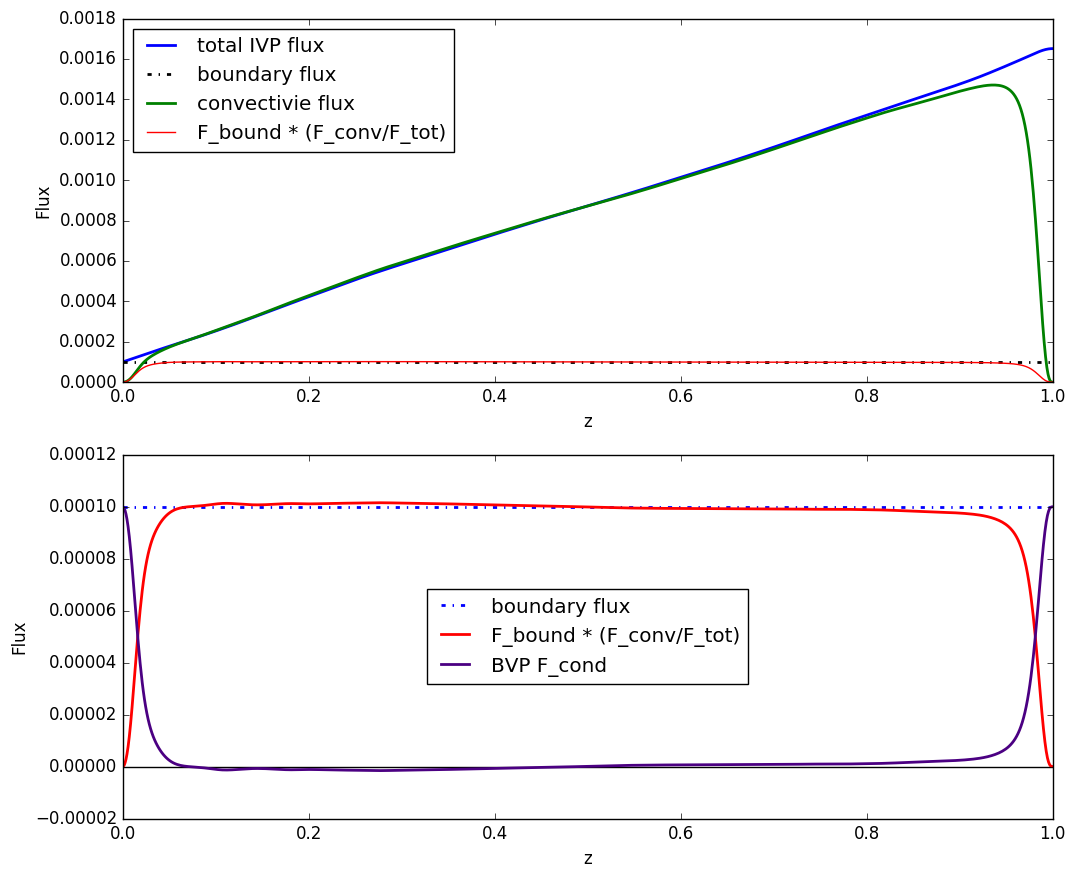
\includegraphics[width=\textwidth]{./figs/bvp_fluxes.png}
\caption{(top) The evolved fluxes from a 2-D rayleigh-benard convection experiment.  The upper
(fixed temp) boundary is leaking out much more flux than the bottom boundary (fixed flux) supplies
while the atmosphere equilibrates.  However, we know that the evolved solution should only carry
the amount of flux supplied at the lower plate.  In the bottom panel, we show the enthalpy flux
in the IVP, divided by the total flux, and then multiplied by the flux at the bottom boundary. This
gives us an idea of what the enthalpy flux should be like in the evolved state, including the
boundary layers.  The corresponding conductive flux that the temperature profile would have to
carry is shown in yellow. \label{fig:flux_fig}}
\end{figure}

\subsection{The actual procedure, and open questions}
So basically what we do is:
\begin{enumerate}
\item Run the IVP to get average fluxes, as in the top panel of Fig. \ref{fig:flux_fig}.
\item Normalize the enthalpy flux profile properly to get the enthalpy flux profile as shown
in the bottom panel of Fig. \ref{fig:flux_fig}
\item Use that normalized enthalpy flux profile as a RHS constant forcing term in the BVP equations
(Eqns. \ref{eqn:RB_BVP_eqns}), and solve for the consistent temperature profile that satisfies
those equations under the proper boundary conditions
\item Update the full fields in the IVP such that the mean pressure and temperature profiles are
the pressure / temperature profiles that come out of the BVP.
\item Run the IVP so that the velocity field relaxes in the presence of the new atmosphere.
\end{enumerate}

This seems to work well.  Open questions:
\begin{enumerate}
\item How long do we average over?  What's the right criterion for having a converged profile?
\item How many times do we need to do the BVP to get to the right answer?  If we get the right
converged profile, I think we're only going to need one BVP.
\item How long does it take the velocity field to fully equilibrate post-BVP?
\item How similar is the BVP final state to the IVP final state?
\end{enumerate}

Note: this is not hard to implement in fully compressible, too!

\section{Extension to Stratified convection and FC equation}
This method is, fortunately, not hard to extend to the fully compressible equations. For
a system whose full energy equation is of the form
$$
\frac{\partial E}{\partial t} + \Div{\bm{F}} = \kappa (\text{IH}),
$$
which is true of both polytropes and internally heated atmospheres, we find that the time
stationary, vertically averaged profile is, once again,
\begin{equation}
\kappa\frac{\partial \angles{T_{1z}}}{\partial z} = 
\frac{\partial}{\partial z}(\angles{\bm{F}_{\text{conv}} - \kappa T_{0z}} - \kappa (IH)
\end{equation}
And, for a properly constructed atmosphere where the initial profile carries the internal
heating, the last two terms of this expression perfectly cancel each other out (at least,
for constant $\kappa$, and for the atmospheres we're worried about right now).  So, with that,
the full set of BVP equations for fully compressible atmospheres is
\begin{equation}
\begin{split}
\frac{\partial T_1}{\partial z} - T_{1z} &= 0 \\
\kappa \frac{\partial T_{1z}}{\partial z} &= \frac{\partial \bm{F}_{\text{conv}}}{\partial z} \\
T_0 \partial_z \rho_1 + T_1 \partial_z \rho_0 + \rho_0 T_{1z} + \rho_1 T_{0z} &= - T_1 \partial_z \rho_1 - \rho_1 T_{1z} \\
\frac{\partial M_1}{\partial z} - \rho_1 &= 0.
\label{eqn:FC_BVP_eqns}
\end{split}
\end{equation}
Here the first two equations are just the energy equation, the third equation is that the
fluctuating components must be in hydrostatic equilibrium ($\grad P = \grad (\rho T) = 
\rho \grad T + T \grad \rho = 0$, and assuming that the background is in hydrostatic equilibrium
such that gravity drops out of the system), and the fourth equation is our mass conservation equation.
This requires four boundary conditions: two thermal ones (fixed flux bot, fixed temp top), and
two mass ones ($M_1 = 0$ at top and bottom).  Once again, by specifying the appropriate profile
for the convective flux, the rest of the atmosphere follows.  This is also nice, because this
formulation should also work with minor tweaks for more complicated forms of $\kappa$.




\end{enumerate}
\end{document}
